\documentclass[a4paper, 10pt, final, garamond]{book}
\usepackage{cours-preambule}
\graphicspath{{./figures/}}

\makeatletter
\renewcommand{\@chapapp}{Contr\^ole de connaissances}
\makeatother

\toggletrue{student}
% % \HideSolutionstrue
% \toggletrue{corrige}
\renewcommand{\mycol}{black}

\begin{document}
\setcounter{chapter}{13}

\chapter{Cinématique et dynamique du point\ifstudent{ (14')}}

\begin{enumerate}[label=\sqenumi]
	\nitem{2}%
	Donner les valeurs de $\Delta{\f_{1/2}(\Mr)}$ et de
	$\Delta{L_{2/1}(\Mr)}$ donnant des interférences constructives et destructives
	pour $\Delta{\f_0}=0$.
	\smallbreak
	\vspace{-30pt}
	\psw{
		\begin{gather*}
			\Delta\f_{1/2}(\Mr) = 2p\pi
			\stm{\Lra}
			\boxed{\Delta{L}_{2/1}(\Mr) = p\lambda}
			\qqet
			\Delta\f_{1/2}(\Mr) = (2p+1)\pi
			\stm{\Lra}
			\boxed{\Delta{L}_{2/1}(\Mr) = \left(p+\frac{1}{2}\right)\lambda}
		\end{gather*}
	}
	\vspace{-15pt}
	\nitem{2}%
	Soient deux points A et B de masses respectives $m_A$ et $m_B$. Exprimer et
	représenter la force d'attraction gravitationnelle de B sur A.
	\smallbreak
	\noindent
	\begin{minipage}{.6\linewidth}
		\psw{
			\vspace{-15pt}
			\[
				\Ff_{g,\rm B\ra A} \stm{=} -\Gc \frac{m_Am_B}{\rm BA^2}\ur
				\qavec
				\ur = \frac{\vv{\rm BA}}{\rm BA}
			\]
			\vspace{-15pt}
		}
	\end{minipage}
	\hfill
	\noindent
	\begin{minipage}{.39\linewidth}
		\begin{center}
			\sswitch{
				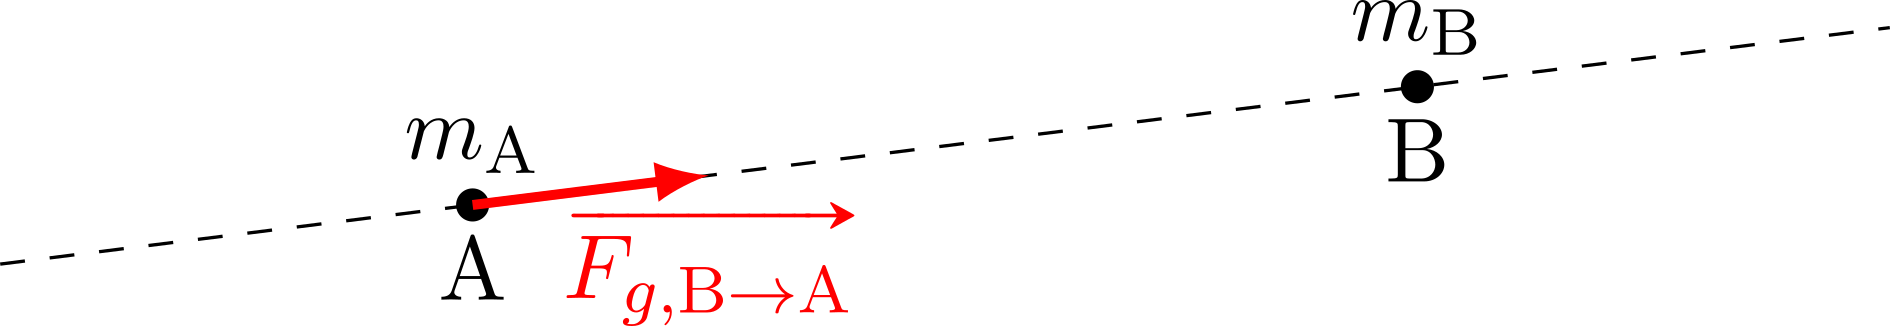
\includegraphics[width=.80\linewidth, draft=true]{fg}
			}{
				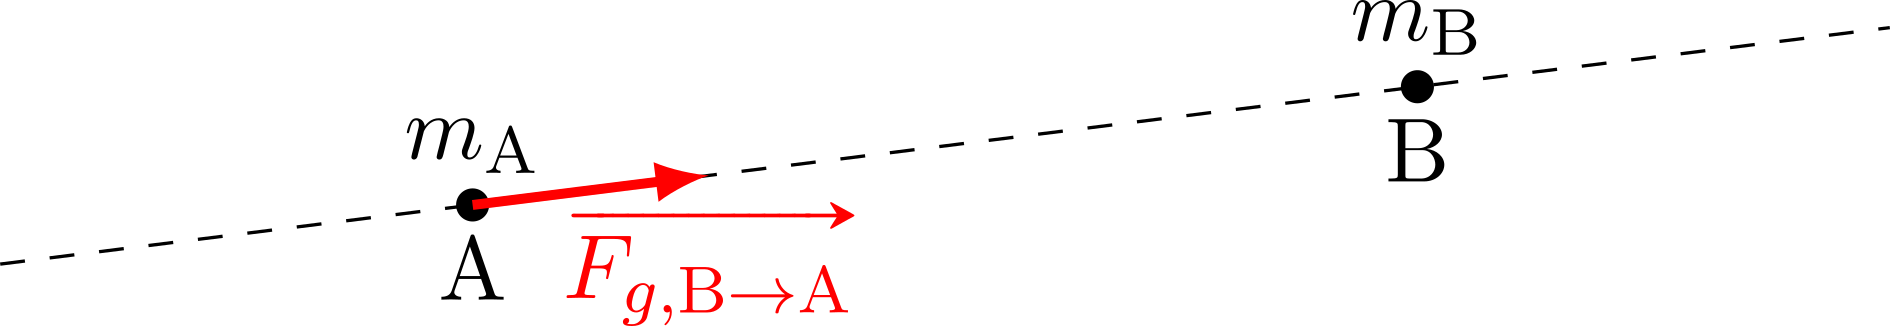
\includegraphics[width=.80\linewidth]{fg}
			}
			\captionof{figure}{Interaction gravitationnelle\protect\pt{1}.}
		\end{center}
	\end{minipage}
	\vspace{-15pt}
	\nitem{3}%
	Énoncer les trois lois de \textsc{Newton}. On travaille avec un système
	ouvert.
	\smallbreak
	\vspace{-15pt}
	\psw{
		\begin{enumerate}
			\litem{20pt}{\pt{1}}
			$\exists \Rc$ galiléens $: (\forall \Mr ~|~ \sum \Ff_{\ext\to\Mr} =
				\of)$, $\Mr$ est soit au repos, soit en translation rectiligne
			uniforme~;
			\litem{20pt}{\pt{1}} $\dv{\pf\Rg(\Mr)}{t} = \sum \Ff_{\ext\to\Mr}$~;
			\litem{20pt}{\pt{1}} $\forall (\Mr_1,\Mr_2), \Ff_{1\to2} = -\Ff_{2\to 1}$.
		\end{enumerate}
	}
	\nitem{4}%
	Donner les \textbf{deux expressions} donnant la position du centre
	d'inertie d'un ensemble de points. Démontrer le lien entre la quantité de
	mouvement d'un ensemble de points et la vitesse du centre d'inertie. Pourquoi
	applique-t-on le PFD avec uniquement les forces extérieures au système~?
	Répondre en français.
	\smallbreak
	\psw{
		\[
			\boxed{\vv{\rm OG} = \sum_i \frac{m_i}{m_{\tot}} \vv{{\OMr}_i}}
			\stm{\Lra}
			\boxed{\sum_i m_i \vv{\rm GM_i} = \of }
		\]
		\begin{gather*}
			\beforetext{Or,}
			\pf\Rg(\Sc) \stm{=} \sum_i \pf\Rg(\Mr_i)
			\qet
			\vf\Rg(\Gr) = \dv{\vv{\rm OG}}{t} = \frac{1}{m_{\tot}}
			\sum_i m_i \dv{{\OM}_i}{t}
			\Lra
			\boxed{\pf\Rg(\Sc) \stm[-1]{=} m_{\tot}\vf\Rg(\Gr)}
		\end{gather*}
		Les forces intérieures se compensent d'après la troisième loi de
		\textsc{Newton} \pt{1}.
	}
	\nitem{9}%
	Soit une balle lancée avec une vitesse $\vfo$ faisant un angle $\alpha$ avec
	l'horizontale. On néglige toute autre force que le poids. Faire un schéma puis
	déterminer les équations horaires des composantes sur $\ux$ et $\uy$ du
	mouvement, et déterminer l'équation de la trajectoire. Portez une attention
	particulière à l'établissement du système.
	\smallbreak
	\psw{
		\noindent
		\begin{minipage}[c]{.60\linewidth}
			\begin{enumerate}[label=\sqenumi]
				\bitem{\lit{20pt}{\pt{1}}Système}~:
				\{balle\} dans $\Rc\ind{labo}$ supposé galiléen
				\bitem{\lit{20pt}{\pt{1}}Schéma}~:
				cf.\ figure.
				\bitem{\lit{20pt}{\pt{1}}Modélisation}~:
				repère $(\!\ux,\uy,\uz)$ (cf.\ schéma),
				\smallbreak
				repérage $\OM = x\ux +y\uy$, $\vf = \xp\ux+\yp\uy$, $\af =
					\xpp\ux+\ypp\uy$.
				\bitem{\lit{20pt}{\pt{1}}Conditions initiales}~:
				$\OM (0) = \of$ et
				\smallbreak
				$\vf(0) = v_0\cos(\alpha)\ux+ v_0\sin(\alpha)\uy$
				\bitem{\lit{20pt}{\pt{1}}BdF}~: $\Pf = -mg\uy$
			\end{enumerate}
		\end{minipage}
		\begin{minipage}[c]{0.39\linewidth}
			\begin{center}
				\sswitch{
					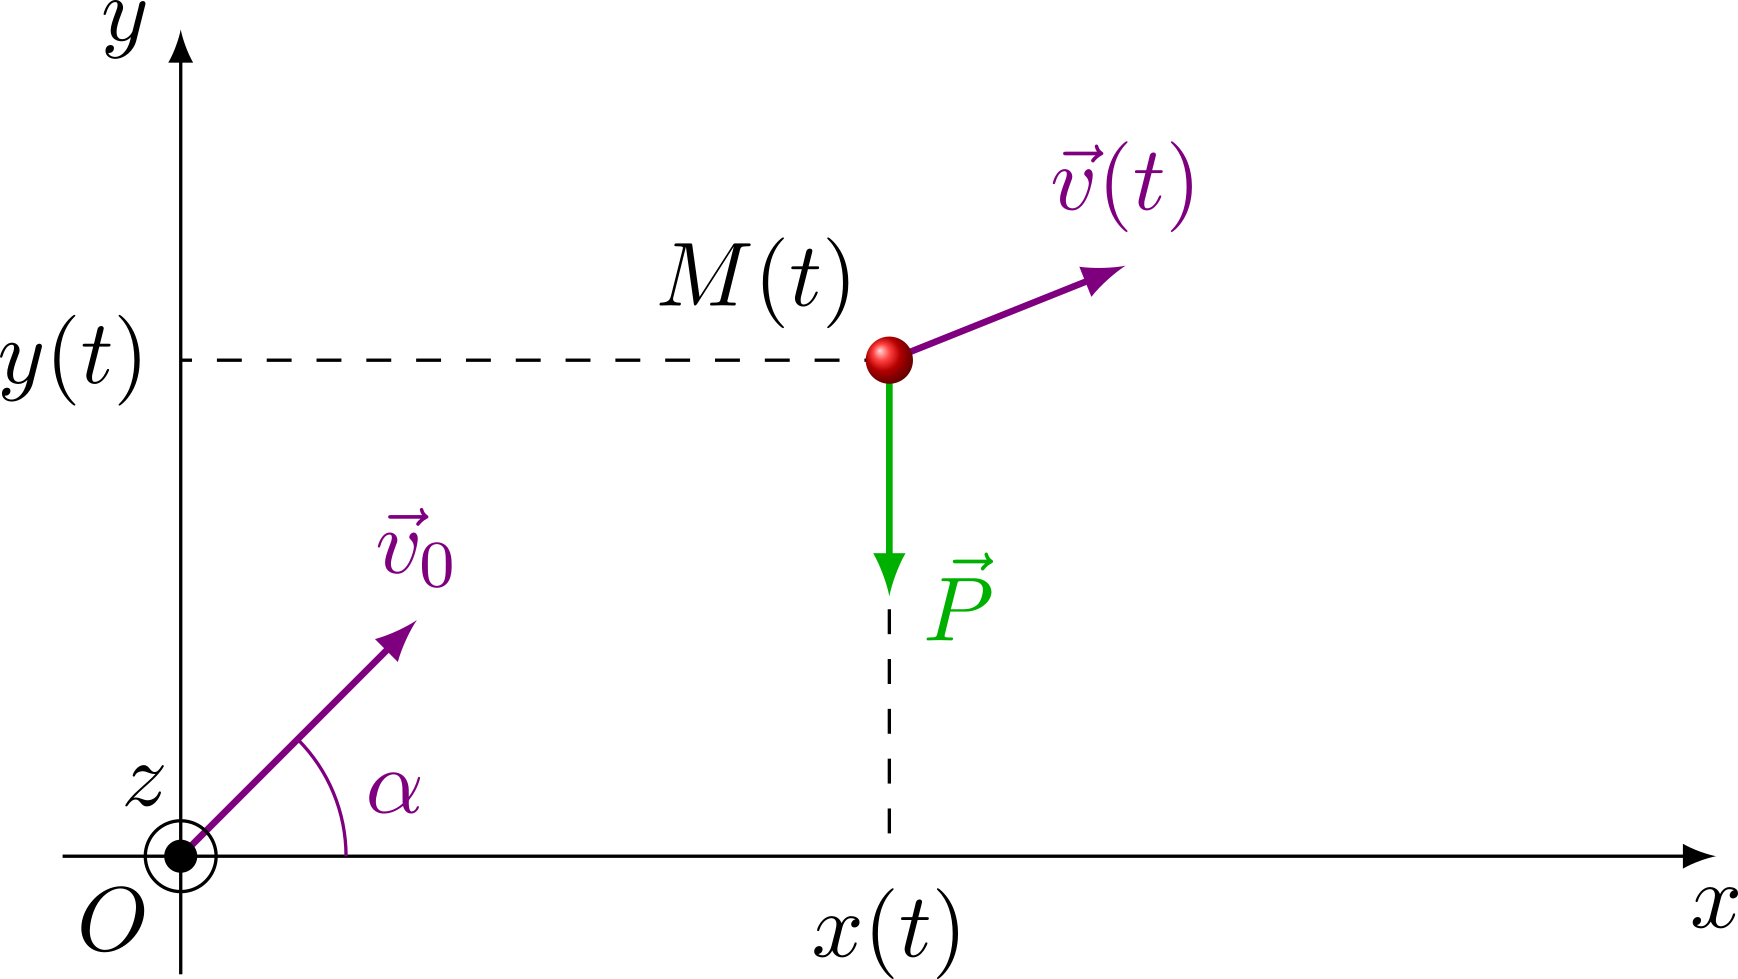
\includegraphics[width=\linewidth, draft=true]{cl_ssf}
				}{
					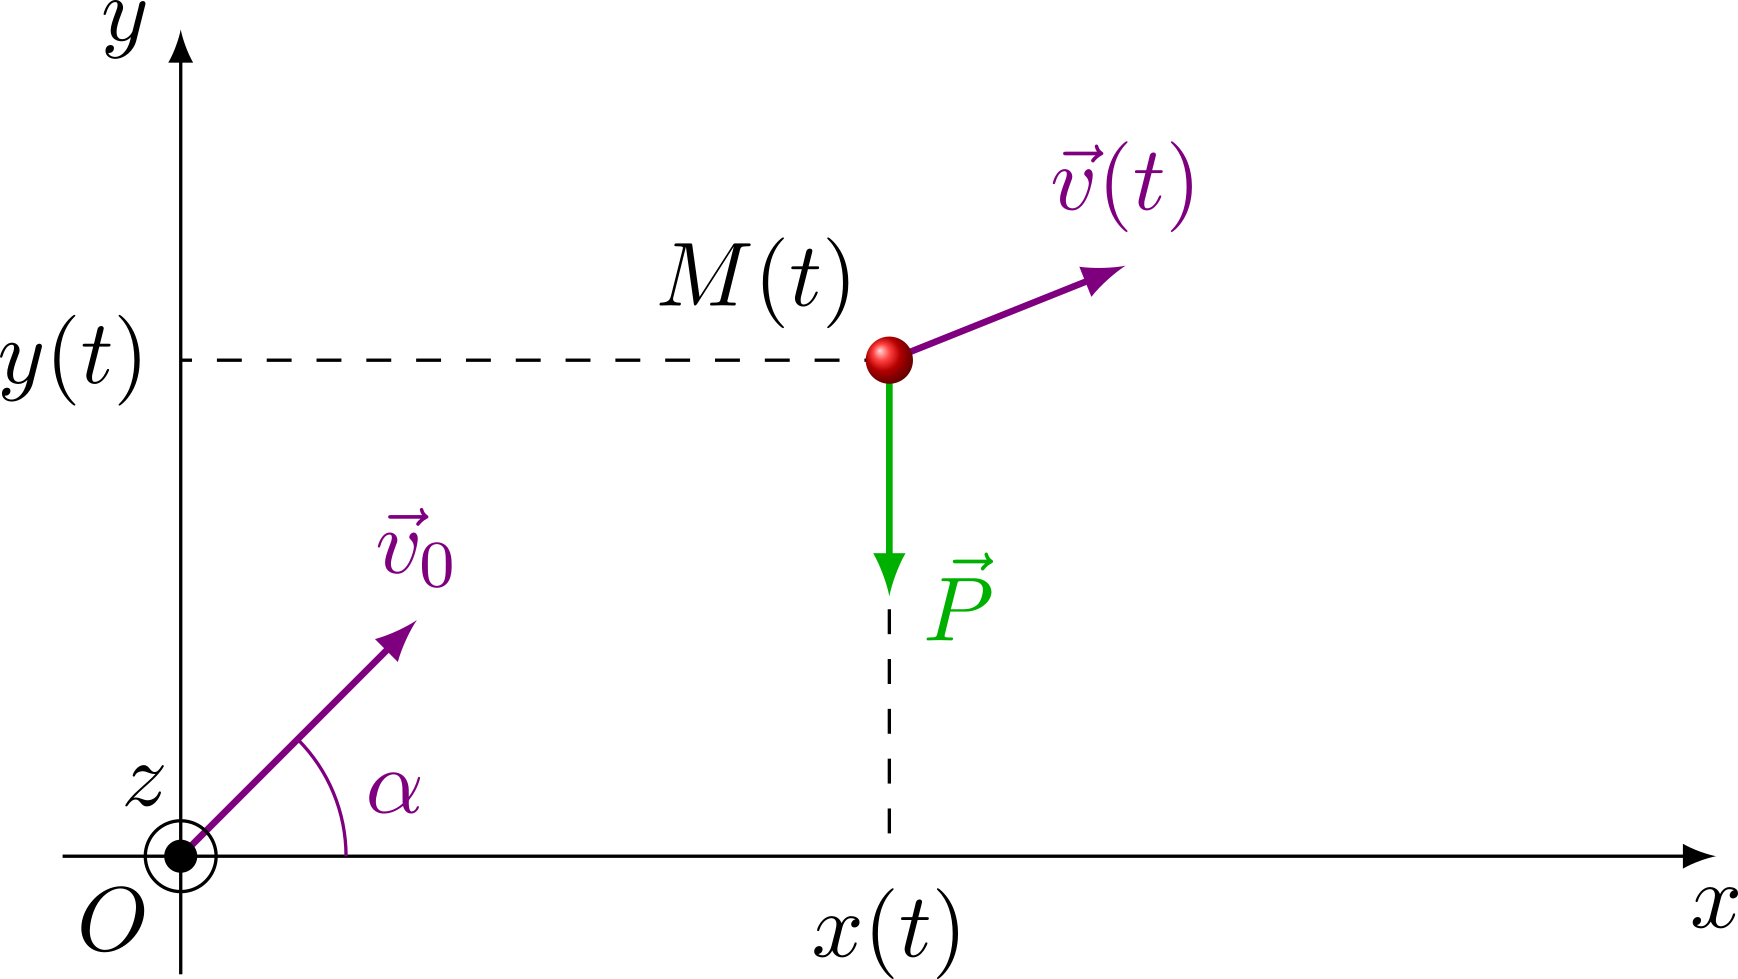
\includegraphics[width=\linewidth]{cl_ssf}
				}
				\vspace{-15pt}
				\captionof{figure}{Chute libre.}
			\end{center}
		\end{minipage}
		\begin{enumerate}[label=\sqenumi, start=6]
			\bitem{PFD}~:
			\vspace{-15pt}
			\[m\af \stm{=} \Pf
				\Lra
				\left\{
				\begin{array}{l}
					\ddot{x}(t) \stm{=} 0 \\
					\ddot{y}(t) = -g
				\end{array}
				\right.
				\Lra
				\left\{
				\begin{array}{l}
					\dot{x}(t) = v_0\cos\alpha \\
					\dot{y}(t) = -gt + v_0 \alpha
				\end{array}
				\right.
				\Lra
				\boxed{
					\left\{
					\begin{array}{l}
						x(t) = v_0t\cos\alpha \\
						y(t) = \DS -\frac{1}{2}gt^2 + v_0t\sin\alpha
					\end{array}
					\right.}
				\pt{1}
			\]
			\begin{gather*}
				\beforetext{Ainsi,}
				t            = \frac{x}{v_0\cos\alpha}
				\Ra
				y(x)         = - \frac{1}{2}g \frac{x^2}{v_0{}^2\cos^2\alpha} +
				v_0\sin\alpha \frac{x}{v_0\cos\alpha}
				\\\Lra
				\boxed{y(x) \stm[-1]{=} - \frac{g}{2v_0{}^2\cos^2\alpha}x^2 + x\tan\alpha}
			\end{gather*}
		\end{enumerate}
	}
	\ifstudent{
		\begin{tikzpicture}[remember picture, overlay]
			\node[anchor=north west, align=left]
			at ([shift={(1.4cm,0)}]current page.north west)
			{\\[5pt]\Large\bfseries Nom~:\\[10pt]\Large\bfseries Prénom~:};
			\node[anchor=north east, align=right]
			at ([shift={(-1.5cm,-17pt)}]current page.north east)
			{\Large\bfseries Note~:\hspace{1cm}/20};
		\end{tikzpicture}
	}
\end{enumerate}
\end{document}
